\section{Models}
Two different models were developed for the sentiment analysis task. The first model is a Recurrent Neural Network (RNN) with Long Short-Term Memory (LSTM) cells, and the second model is a Transformer model.

\subsection{Model 1: RNN-LSTM}
We choose to start with a 'simple' RNN model with LSTM cells. By using a grid search approach over the hyperparameters like the number of hidden units, the number of layers, the dropout rate, etc., we found the following model shown in Table \ref{tab:rnn_lstm_model}, having in total 1,117,734 number of parameters.
\begin{table}[H]
    \vspace*{-0.5cm}
    \centering
    \begin{tabular}{|l|}
    \hline
    Embedding w/ 10,336 \#embeddings (vocab size) and 75 \#embedding dims. \\ \hline
    LSTM w/ 10,336 \#features and 256 \#hidden units in 1 layer \\ \hline
    Dropout w/ 50\% dropout rate \\ \hline
    Linear w/ 256 \#features and 6 \#output classes \\ \hline
    \end{tabular}
    \caption{RNN-LSTM model.}
    \label{tab:rnn_lstm_model}
    \vspace*{-0.8cm}
\end{table}

The model is trained using the AdamW optimizer with a learning rate of 0.001, a batch size of 16. We use the CrossEntropyLoss as the loss function and train the model for 4 epochs. To prevent overfitting, we add a 0.0001 L2-norm penalty to the weights.
\begin{figure}[H]
    \vspace*{0.7cm}
    \centering
    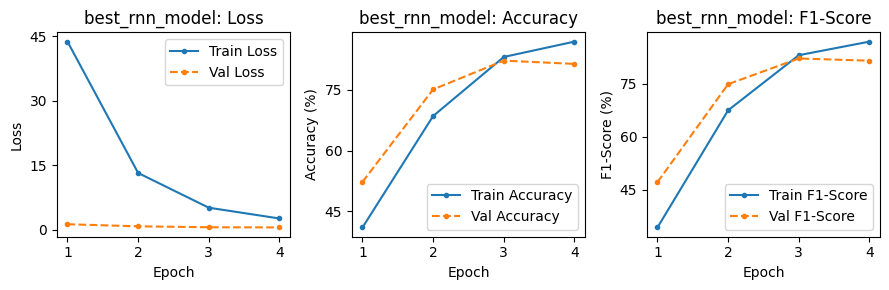
\includegraphics[width=0.6\textwidth]{figures/rnn_scores.png}
    \caption{Training and validation loss, accuracy and F1-score for the RNN-LSTM model.}
    \label{fig:rnn_scores}
    \vspace*{0.7cm}
\end{figure}
From Figure \ref{fig:rnn_scores}, we see we hit the inflection point around 3 epochs, which is why we choose stop the training after 4 epochs.
\begin{table}[H]
    \vspace*{-0.5cm}
    \centering
    \begin{tabular}{|c|c|}
    \hline
    Validation Accuracy & Validation F1-Score \\ \hline
    81.4\% & 81.4\% \\ \hline
    \end{tabular}
    \caption{RNN-LSTM model performance on validation set.}
    \label{tab:rnn_lstm_model}
    \vspace*{-0.8cm}
\end{table}